\documentclass{fkssolpub}

\usepackage[czech]{babel}
\usepackage{fontspec}
\usepackage{fkssugar}
\usepackage{amsmath}
\usepackage{graphicx}

\author{Ondřej Sedláček}
\school{Gymnázium Oty Pavla} 
\series{2j}
\problem{6} 

\begin{document}

\begin{figure}
	\begin{center}
		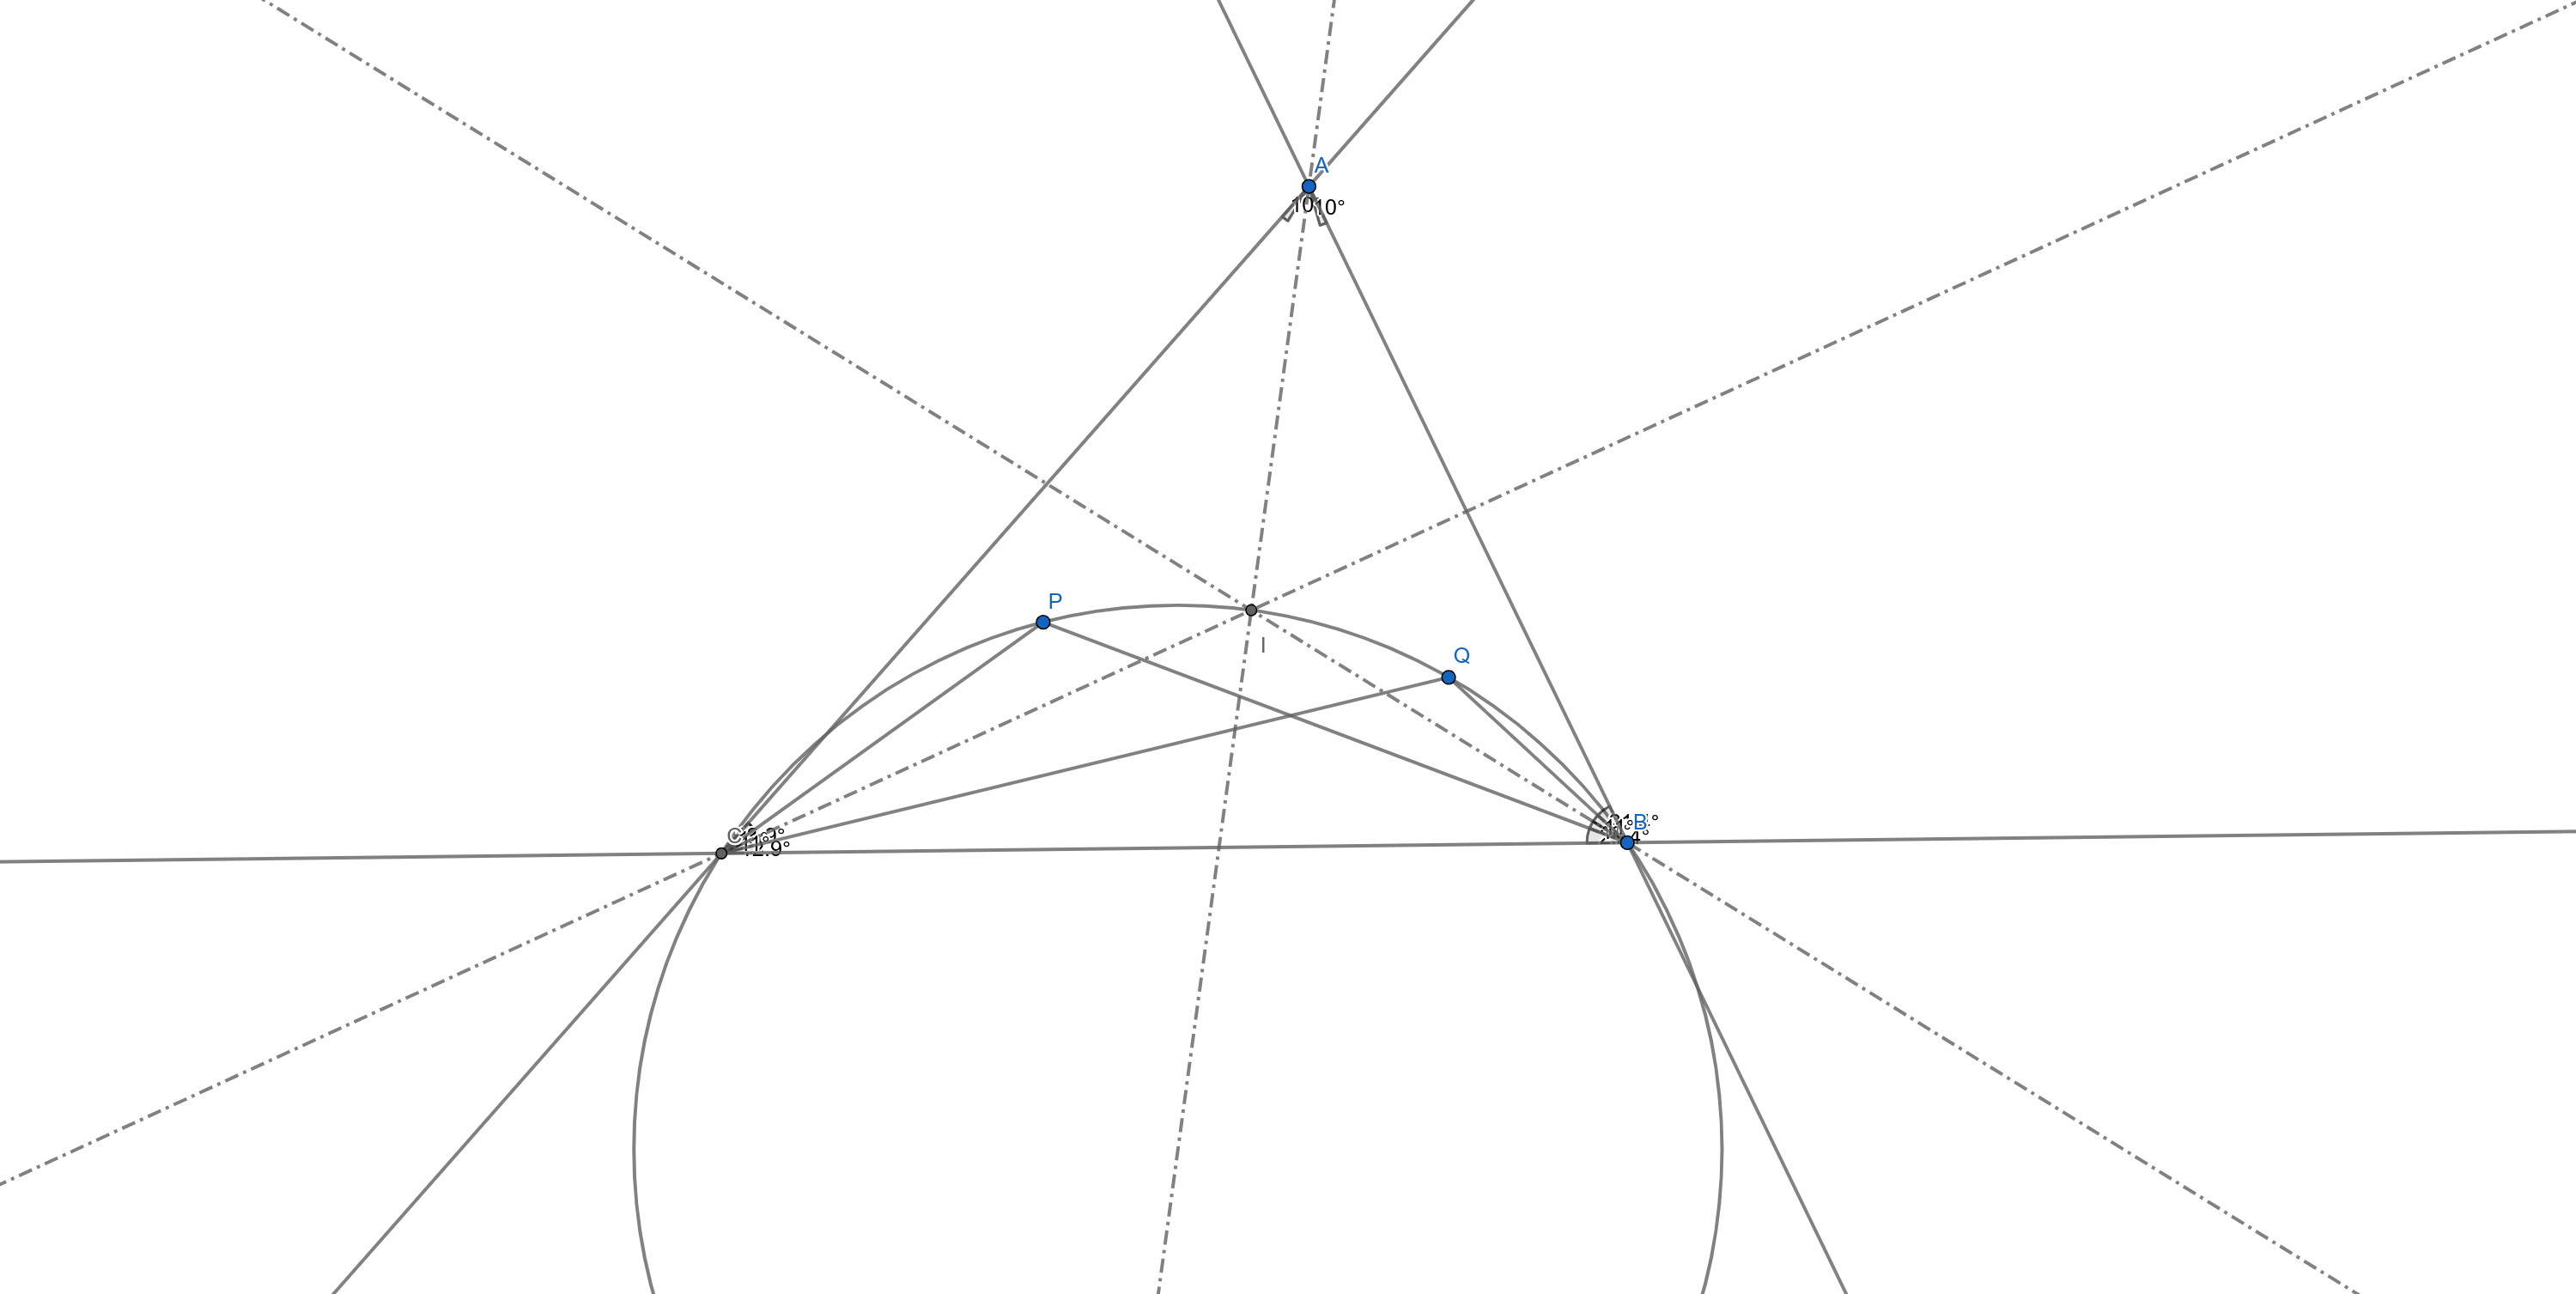
\includegraphics[width=0.95\textwidth]{6-fig.png}
	\end{center}
	\caption{Konstrukce řešení}
	\label{fig:sol}
\end{figure}

Z podmínky $|AP| = |AQ|$ víme, že trojúhelník $APQ$ je rovnoramenný a že osa
strany $PQ$ je osa úhlu při vrcholu $A$ díky vlastnostem kamarádů.

Teď dokážeme, že vepsiště trojúhelníku $ABC$ je jak Švrčkovým bodem trojúhelníku
$CPQ$, tak i $BPQ$. Víme, že osa úhlu $\angle ACB$ je stejná jako osa úhlu
$\angle PCQ$ a že osa úhlu $\angle CAB$ je osa strany $PQ$. Z toho vyplývá,
že průsečík těchto přímek, tedy vepsiště trojúhelníku $ABC$, je Švrčkovým
bodem trojúhelníku $CPQ$. Obdobně to dokážeme pro $BPQ$.

Odtud už můžeme ukázat, že $|\angle PCQ| = |\angle PBQ|$:

\[
	|\angle PCQ| = |\angle PCI| + |\angle ICQ| = |\angle IPQ| + |\angle PQI|
	= |\angle PBI| + |\angle IBQ| = |\angle PBQ|
\]

Z toho vyplývá, že čtyřúhelník $PQBC$ je tětivový, tedy body $P, Q, B, C$
leží na jedné kružnici. Q. E. D.

\end{document}
